\Variant{07.03.2026 (1-smena)}
\QQ{1}{Agar $m=24^3\cdot6^{12}\cdot20^3$ bölsa, $\dfrac{m^2}{2^n}$ kasrning qiymati natural son böladigan $n$ ning eng katta qiymatini toping.
\Opts{$54$}{$48$}{$27$}{$60$}}
\QQ{2}{Agar $a=\lg3$, $b=\cos3$, $c=\ln3$ bölsa, ifodani soddalaştiring:
\[\frac{|a-b|+|b-c|-|a-c|}{|a+b|+|b-c|-|c+a|}\]
\Opts{$\dfrac{b+a}b$}{$\dfrac{b-a}{b+a}$}{$\dfrac{a-b}a$}{$-\dfrac{b-a}{b+a}$}}
\QQ{3}{Muğombir soddadilga: «Köprikdan har bir ötişingda çöntagingdagi pulni $2$ marta oşirib beraman, lekin sen har safar ötganingda menga $36\,000$ söm berasan», — dedi. Soddadil köprikdan $3$ marta ötgandan söng uning puli tugadi. Boşida soddadilning neça söm puli bölgan?
\Opts{$45\,000$}{$36\,000$}{$32\,000$}{$31\,500$}}
\QQ{4}{Suv va neftdan iborat $60$ litr aralaşma tarkibidan $15$ litr neft ajratib olindi. Qolgan aralaşma tarkibida $4\%$ neft qoldi. $60$ litr aralaşmaning tarkibida neça foiz neft bölgan?
\Opts{$28\%$}{$20\%$}{$24\%$}{$26\%$}}
\QQ{5}{Soddalaştiring:
\[\frac{\left(a^2\right)^{-3}\cdot\left(-a^2\right)^7}{\left(-a^3\right)^2}\]
\Opts{$-a^2$}{$a^2$}{$a^3$}{$a^{-3}$}}
\QQ{6}{Hisoblang:
\[\frac1{\sqrt2+2}-\frac1{2-\sqrt2}-\sqrt2\]
\Opts{$-\sqrt2$}{$-2\sqrt2$}{$2\sqrt2$}{$\sqrt2$}}
\QQ{7}{Hisoblang:
\[\frac{8\left(\sqrt3-\sqrt{15}\right)}{\sqrt3+\sqrt7+\sqrt{11}+\sqrt{15}}+\frac{8\left(\sqrt3-\sqrt{15}\right)}{\sqrt3-\sqrt7-\sqrt{11}+\sqrt{15}}\]
\Opts{$1$}{$-9\sqrt5-3\sqrt{11}$}{$-9\sqrt5+2\sqrt{11}$}{$9\sqrt5+3\sqrt{77}$}}
\QQ{8}{$\log_{12}162$, $\log_{12}x$, $\log_{12}y$, $\log_{12}z$, $\log_{12}1250$ sonlari arifmetik progressiyaning ketma-ket hadlari bölsa, $z-x-y$ ning qiymatini toping.
\Opts{$-30$}{$20$}{$30$}{$570$}}
\QQ{9}{Maxraji $q<1$ bölgan geometrik progressiyada $b_1+b_2+b_3=21$ va $b_1\cdot b_2\cdot b_3=216$ bölsa, $S_5$ ni toping.
\Opts{$23\dfrac14$}{$93$}{$22\dfrac12$}{$45$}}
\QQ{10}{Soddalaştiring:
\[\frac{a^3-b^3}{(2a+b)^2-3a(a+b)}+\frac{\left(a^2+b\right)\left(b^2+a\right)-ab(ab+1)}{a^2-ab+b^2}\]
\Opts{$2b$}{$2a$}{$2a+2b$}{$2a-2b$}}
\QQ{11}{Agar $a\ge3$ bölsa, ifodani soddalaştiring:
\[\left(\frac{a+\sqrt{a^2-3a}}{a-\sqrt{a^2-3a}}-\frac{a-\sqrt{a^2-3a}}{a+\sqrt{a^2-3a}}\right)\cdot\frac34\]
\Opts{$\sqrt{a^2-3a}$}{$a^2-3a$}{$a^2+3a$}{$\sqrt{a^2+3a}$}}
\QQ{12}{Sonlarni kamayiş tartibida joylaştiring:
\[a=\sin17^\circ,\qquad b=\sin167^\circ,\qquad c=\sin375^\circ\]
\Opts{$a>c>b$}{$b>a>c$}{$c>b>a$}{$c>a>b$}}
\QQ{13}{Tenglamaning $[0;\,4\pi]$ oraliqdagi ildizlari yiğindisini toping:
\[2\left(\sin^2x+\tg^2x\right)+3=4\tg x+2\sqrt2\sin x\]
\Opts{$\dfrac{5\pi}2$}{$\dfrac{9\pi}2$}{$5\pi$}{$9\pi$}}
\QQ{14}{Tenglamaning haqiqiy ildizlari yiğindisini toping:
\[\left(\sqrt{7+4\sqrt3}\right)^x+\left(\sqrt{7-4\sqrt3}\right)^x=14\]
\Opts{$-2$}{$2$}{$-4$}{$0$}}
\QQ{15}{Tenglamani yeçing:
\[\left(\frac23\right)^{\log_3(x+1)}\cdot\left(\frac49\right)^{\log_{\frac19}(x-1)}=\frac23\]
\Opts{$2$}{$4$}{$6$}{$0$}}
\QQ{16}{Tenglamalar sistemasining yeçimlari $(x_1;\,y_1)$, $(x_2;\,y_2)$, \ldots, $(x_n;\,y_n)$ bölsa, $x_1+x_2+\ldots+x_n$ ni toping.
\[\begin{cases}x^2+y^2=34,\\ x+xy+y=7\end{cases}\]
\Opts{$0$}{$6$}{$-2$}{$-8$}}
\QQ{17}{Tenglamaning haqiqiy ildizlari yiğindisini toping:
\[\left(x^2-8x+12\right)\cdot\sqrt{10+3x-x^2}=0\]
\Opts{$5$}{$-2$}{$3$}{$11$}}
\QQ{18}{Tengsizliklar sistemasini yeçing:
\[\begin{cases}\dfrac{36}x-x\le0,\\[2mm] \dfrac{|12-2x|\cdot\left(x^2+5x+25\right)}{|x|-3}\le0\end{cases}\]
\Opts{$(-3;\,3)\cup\{6\}$}{$(-3;\,0)\cup(0;\,6)$}{$(-3;\,0)\cup\{6\}$}{$(-\infty;\,6)\cup(6;\,\infty)$}}
\QQ{19}{Tengsizlikni yeçing:
\[\sqrt{x-11}+\sqrt{12-x}>0\]
\Opts{$(11;\,12)$}{$[11;\,12]$}{$\{11;\,12\}$}{$(-\infty;\,\infty)$}}
\QQ{20}{Agar $f(x)=\begin{cases}8+x, & x<0,\\ 2-x, & x\ge0\end{cases}$ bölsa, $f\Bigl(f\bigl(f(-5)\bigr)\Bigr)$ ni toping.
\Opts{$3$}{$7$}{$5$}{$9$}}
\QQ{21}{Aniq integralni hisoblang:
\[\int_3^6\frac{x+1}{x^2+x-6}\,dx\]
\Opts{$\dfrac25\ln6$}{$\dfrac45\ln6$}{$\dfrac45\ln12$}{$\dfrac25\ln12$}}
\QQ{22}{Agar $f(x)=\dfrac{x+x^2+x^3+\ldots+x^{2024}}{x+x^2+x^3+\ldots+x^{1012}}$ bölsa, $f'(1)$ ni toping.
\Opts{$1$}{$-1$}{$-1012$}{$1012$}}
\QQ{23}{Rasmda bitta töğri çiziqqa urinuvçi $O_1$ va $O_2$ markazli aylanalar tasvirlangan. $AB$ — aylanalarning umumiy urinmasi. Agar $O_1$ aylana radiusi $5$ ga, $O_2$ aylana radiusi $2$ ga teng va $O_1O_2=11$ bölsa, $AB$ kesmani toping.
\qfig{\begin{tikzpicture}[scale=0.3,font=\small]
\coordinate (O1) at (0,5); \coordinate (O2) at (10.583,2);
\draw (-6,0)--(13.5,0); \draw (O1) circle (5); \draw (O2) circle (2);
\coordinate (A) at ($(O1)+(58.34:5)$); \coordinate (B) at ($(O2)+(58.34:2)$);
\draw ($(A)!-0.15!(B)$)--($(B)!-0.3!(A)$); \draw[dashed] (O1)--(O2); \draw (O1)--(0,0); \draw (O2)--(10.583,0);
\fill (O1) circle (4pt); \fill (O2) circle (4pt); \fill (A) circle (4pt); \fill (B) circle (4pt);
\node[above] at (A) {$A$}; \node[above right] at (B) {$B$}; \node[above left] at (O1) {$O_1$}; \node[above] at (O2) {$O_2$};
\node[left] at (0,2.5) {$5$}; \node[right] at (10.583,0.9) {$2$}; \node[below] at (5.5,3.2) {$11$}; \node[above right] at ($(A)!0.5!(B)$) {$x$};
\end{tikzpicture}}
\Opts{$4\sqrt7$}{$\sqrt{117}$}{$\sqrt{130}$}{$3\sqrt7$}}
\QQ{24}{$f(x)=x^2-2ax-a-6$ funksiya grafigining $Ox$ öqini kesib ötuvçi nuqtalari orasidagi masofa $10$ ga teng bölsa, $a$ ning qiymatlari yiğindisini toping (agar u bitta bölsa, şu sonni toping).
\Opts{$-1$}{$4$}{$-6$}{$10$}}
\QQ{25}{$ABC$ uçburçakda $AD$ — bissektrisa ($D\in BC$), $E\in AC$ va $|AD|=|AC|$, $|AE|=|DE|=|DC|$. $DF\perp AB$ ($F\in AB$), $FL$ — $BFD$ burçakning bissektrisasi ($L\in BC$). $\angle FLB=\beta$ ni toping.
\qfig{\begin{tikzpicture}[scale=3.4,font=\small]
\coordinate (A) at (0,0); \coordinate (C) at (1,0); \coordinate (B) at (0.5,1.539); \coordinate (D) at (0.809,0.588); \coordinate (E) at (0.618,0); \coordinate (F) at (0.25,0.769); \coordinate (L) at (0.679,0.988);
\draw (A)--(B)--(C)--cycle; \draw (A)--(D); \draw (D)--(E); \draw (D)--(F); \draw (F)--(L);
\draw ($(F)!0.07!(B)$)--($(F)!0.07!(B)+(F)!0.07!(D)-(F)$)--($(F)!0.07!(D)$);
\draw ($(L)+(-108:0.09)$) arc[start angle=-108,end angle=-153,radius=0.09]; \node at ($(L)+(-130:0.15)$) {$\beta$};
\draw ($(A)+(0:0.12)$) arc[start angle=0,end angle=36,radius=0.12]; \draw ($(A)+(36:0.15)$) arc[start angle=36,end angle=72,radius=0.15];
\draw (0.309,-0.02)--(0.309,0.02); \draw ($(E)!0.5!(D)+(-0.02,0.006)$)--($(E)!0.5!(D)+(0.02,-0.006)$); \draw ($(D)!0.5!(C)+(-0.019,-0.006)$)--($(D)!0.5!(C)+(0.019,0.006)$);
\node[below left] at (A) {$A$}; \node[above] at (B) {$B$}; \node[below right] at (C) {$C$}; \node[right] at (D) {$D$}; \node[below] at (E) {$E$}; \node[left] at (F) {$F$}; \node[right] at (L) {$L$};
\end{tikzpicture}}
\Opts{$90^\circ$}{$99^\circ$}{$100^\circ$}{$108^\circ$}}
\QQ{26}{$ABC$ muntazam uçburçakning tomoni $8$ ga teng. $AD$ kesma $BC$ asosni $5$ va $3$ ga teng kesmalarga ajratadi. $ADC$ va $ABD$ uçburçaklarga içki çizilgan doiralar yuzlari yiğindisini toping.
\qfig{\begin{tikzpicture}[scale=0.42,font=\small]
\coordinate (C) at (0,0); \coordinate (B) at (8,0); \coordinate (A) at (4,6.928); \coordinate (D) at (5,0);
\fill[qfill] (3,1.732) circle (1.732); \fill[qfill] (6,1.1547) circle (1.1547);
\draw (A)--(B)--(C)--cycle; \draw (A)--(D); \draw (3,1.732) circle (1.732); \draw (6,1.1547) circle (1.1547);
\node[above] at (A) {$A$}; \node[below left] at (C) {$C$}; \node[below right] at (B) {$B$}; \node[below] at (D) {$D$};
\node[above left] at (2,3.464) {$8$}; \node[above right] at (6,3.464) {$8$}; \node[below] at (2.5,0) {$5$}; \node[below] at (6.5,0) {$3$};
\end{tikzpicture}}
\Opts{$\dfrac{14\pi}3$}{$14\pi$}{$\dfrac{13\pi}3$}{$6\pi$}}
\QQ{27}{$ABCD$ trapetsiyaning ($BC\parallel AD$) diagonallari $O$ nuqtada kesişadi. $BOC$ uçburçak yuzi $3$ ga teng. Agar $\dfrac{S_{BOC}}{S_{COD}}=\dfrac13$ bölsa, $AOB$ uçburçak yuzini toping.
\qfig{\begin{tikzpicture}[scale=0.75,font=\small]
\coordinate (A) at (0,0); \coordinate (D) at (6,0); \coordinate (B) at (1,2); \coordinate (C) at (3,2); \coordinate (O) at (2.25,1.5);
\fill[qfill] (A)--(B)--(O)--cycle;
\draw (A)--(B)--(C)--(D)--cycle; \draw (A)--(C); \draw (B)--(D);
\node[below left] at (A) {$A$}; \node[above left] at (B) {$B$}; \node[above right] at (C) {$C$}; \node[below right] at (D) {$D$}; \node[below] at (2.25,1.38) {$O$};
\end{tikzpicture}}
\Opts{$12$}{$27$}{$9$}{$15$}}
\QQ{28}{Muntazam oltiburçakning tomoni $1$ ga teng. Uning tomonlari örtalari tutaştirilib, yangi oltiburçak hosil qilindi. Hosil bölgan oltiburçak bilan ham şu jarayon çeksiz davom ettirildi. Barça oltiburçaklar yuzlarining yiğindisini toping.
\qfig{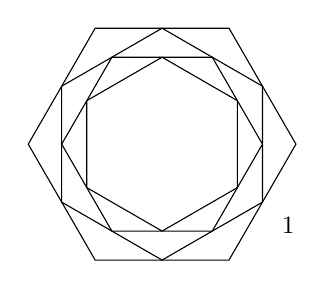
\begin{tikzpicture}[scale=1.7,font=\small]
\draw (1.0000,0.0000) -- (0.5000,0.8660) -- (-0.5000,0.8660) -- (-1.0000,0.0000) -- (-0.5000,-0.8660) -- (0.5000,-0.8660) -- cycle;
\draw (0.7500,0.4330) -- (0.0000,0.8660) -- (-0.7500,0.4330) -- (-0.7500,-0.4330) -- (-0.0000,-0.8660) -- (0.7500,-0.4330) -- cycle;
\draw (0.3750,0.6495) -- (-0.3750,0.6495) -- (-0.7500,0.0000) -- (-0.3750,-0.6495) -- (0.3750,-0.6495) -- (0.7500,-0.0000) -- cycle;
\draw (0.0000,0.6495) -- (-0.5625,0.3248) -- (-0.5625,-0.3248) -- (-0.0000,-0.6495) -- (0.5625,-0.3248) -- (0.5625,0.3248) -- cycle;
\node[below right] at (-30:0.95) {$1$};
\end{tikzpicture}}
\Opts{$10$}{$15$}{$6\sqrt3$}{$9\sqrt3$}}
\QQ{29}{$A(6;\,4;\,-2)$, $B(x;\,y;\,0)$ nuqtalar va $\overrightarrow{CD}(4;\,-3;\,1)$ vektor berilgan. $\overrightarrow{AB}$ va $\overrightarrow{CD}$ vektorlar kollinear bölsa, $\overrightarrow{AB}$ ning koordinatalari yiğindisini toping.
\Opts{$4$}{$12$}{$-12$}{$-4$}}
\QQ{30}{Rombning diagonallari $60$ va $80$ ga teng. Romb tekisligiga tegişli bölmagan $P$ nuqtadan rombning diagonallari kesişgan nuqtasiga romb tekisligiga perpendikulyar bölgan, uzunligi $45$ ga teng kesma tuşirilgan. $P$ nuqtadan rombning tomonigaça bölgan masofani toping.
\Opts{$51$}{$24$}{$36$}{$40$}}
\QQ{31}{$A=\{1;\,2;\,3;\,4;\,5;\,6\}$ töplam berilgan. Töplamning neçta qism töplamida $3$ yoki $5$ elementlaridan kamida bittasi qatnaşadi?
\Opts{$64$}{$48$}{$32$}{$16$}}
\QQ{32}{$C_n^4-C_n^3=14$ bölsa, $C_n^2$ ni toping.
\Opts{$14$}{$21$}{$24$}{$28$}}
\QQ{33}{\Moslash{Silindrning balandligi $8$ ga, töla sirti $232{,}5\pi$ ga teng. Quyidagilarni hisoblang.
\par\centering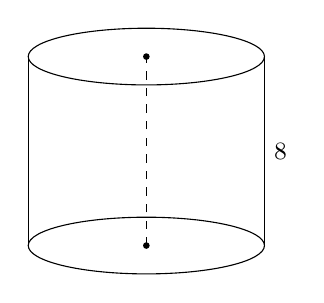
\begin{tikzpicture}[scale=0.3,font=\small]
\draw (0,0) ellipse (5 and 1.2); \draw (0,8) ellipse (5 and 1.2); \draw (-5,0)--(-5,8); \draw (5,0)--(5,8);
\draw[dashed] (0,0)--(0,8); \fill (0,0) circle (4pt); \fill (0,8) circle (4pt); \node[right] at (5,4) {$8$};
\end{tikzpicture}}{A) $\dfrac{\sqrt{161}}2$\par B) $\dfrac{\sqrt{161}}4$\par C) $\dfrac{17}2$\par D) $\dfrac{3\sqrt{21}}2$\par E) $\dfrac{3\sqrt{21}}4$\par F) $\dfrac{19}2$}{Uçlari silindrning turli asoslari aylanalarida yotgan $10$ ga teng kesma berilgan. Silindr öqidan şu kesmagaça bölgan masofani toping.}{Silindr öqiga parallel kesim kvadratdan iborat. Silindr öqidan şu kesimgaça bölgan masofani toping.}{Silindrga taşqi çizilgan şar radiusini toping.}}
\QQ{36}{Tenglamalar sistemasi berilgan:
\[\begin{cases}x^2+y^2-2(x-y)a=9-6a-a^2,\\ x^2+y^2+2(3x+4y)a=1-2a-24a^2\end{cases}\]
\AB{Tenglamalar sistemasi yagona haqiqiy yeçimga ega böladigan $a$ ning neçta qiymati mavjud?}{Tenglamalar sistemasi yagona haqiqiy yeçimga ega böladigan $a$ ning eng katta qiymatini toping.}}
\QQ{37}{Tenglamani yeçing:
\[\sin^{10}x+\cos^{10}x=\frac{29}{16}\cos^42x\]
\AB{Tenglamaning eng kiçik musbat ildizini toping.}{Tenglamaning $[-\pi;\,\pi]$ oraliqdagi ildizlari yiğindisini toping.}}
\QQ{38}{$f(x)=a|x+b|+c$ va $g(x)=kx+l$ funksiyalar grafiklari $(6;\,1)$ nuqtada kesişadi. $f(x)$ funksiya $(2;\,3)$ nuqtada maksimumga erişadi. $(-\infty;\,2)$ oraliqda funksiyalar grafiklari özaro parallel.
\qfig{\begin{tikzpicture}[scale=0.5,font=\small]
\draw[-{Stealth[length=4pt]}] (-4,0)--(9,0) node[right] {$x$}; \draw[-{Stealth[length=4pt]}] (0,-4.5)--(0,5) node[left] {$y$};
\draw[thick] (-4,0)--(2,3)--(9,-0.5); \draw (-3,-3.5)--(9,2.5);
\fill (2,3) circle (3pt); \fill (6,1) circle (3pt);
\node[above] at (2,3) {$(2;\,3)$}; \node[above] at (6,1.2) {$(6;\,1)$}; \node[above left] at (-2.6,1) {$f(x)$}; \node[below right] at (7.5,1.5) {$g(x)$}; \node[below left] at (0,0) {$O$};
\end{tikzpicture}}
\AB{$3\cdot\dfrac{a+b+c}{k+l}$ ni toping.}{$(-\infty;\,2)$ oraliqdagi $f(x)$ va $g(x)$ funksiyalar grafiklari orasidagi eng qisqa masofani toping.}}
\QQ{39}{$f(x)=\dfrac{x^5}{40}+\dfrac{x^4}8-\dfrac{x^3}6-x^2+2$ funksiya berilgan.
\AB{Funksiyaning lokal maksimum nuqtalari sonini toping.}{$f(x)$ funksiyaning $[-5;\,2]$ kesmadagi eng katta qiymatini toping.}}
\QQ{40}{Rasmda $f(x)=ax^2+bx+c$ va $g(x)=kx+l$ funksiyalar grafiklari tasvirlangan. $f(x)$ funksiya grafigi $Ox$ öqini $(-6;\,0)$ va $(2;\,0)$ nuqtalarda kesib ötadi. $g(x)$ funksiya grafigi $f(x)$ funksiya grafigi bilan $(-4;\,3)$ va $(2;\,0)$ nuqtalarda kesişadi.
\qfig{\begin{tikzpicture}[scale=0.5,font=\small]
\fill[qfill] plot[domain=-4:2,samples=50] (\x,{-(\x+6)*(\x-2)/4})--cycle;
\draw[-{Stealth[length=4pt]}] (-8,0)--(4.5,0) node[right] {$x$}; \draw[-{Stealth[length=4pt]}] (0,-2.8)--(0,5.5) node[left] {$y$};
\draw[thick,domain=-6.6:2.5,samples=80] plot (\x,{-(\x+6)*(\x-2)/4});
\draw[domain=-5.2:3.6,samples=2] plot (\x,{-\x/2+1});
\fill (-4,3) circle (3pt); \fill (2,0) circle (3pt); \fill (-6,0) circle (3pt);
\node[left] at (-4.2,3.2) {$A(-4;\,3)$}; \node[below left] at (-6,0) {$-6$}; \node[below left] at (2,0) {$2$};
\node[below right] at (3.6,-0.8) {$g(x)$}; \node[below left] at (2.5,-1.06) {$f(x)$};
\end{tikzpicture}}
\AB{$\dfrac{a+b+c}{k+l}$ ning qiymatini toping.}{Böyalgan soha yuzini toping.}}
\QQ{41}{Töğri burçakli uçburçakning töğri burçagi uçidan gipotenuzaga balandlik va bissektrisa tuşirilgan. Balandlik va bissektrisa uzunliklari mos ravişda $6$ va $8$ ga teng.
\AB{Uçburçak yuzini toping.}{Uçburçak gipotenuzasini toping.}}
\QQ{42}{$ABCD$ kvadratning $AC$ diagonalidan $E$ nuqta, $CD$ tomonidan $F$ nuqta olingan va $BE$ hamda $EF$ kesmalar özaro perpendikulyar. Agar $AE=1$ va $BE=\sqrt3+1$ bölsa,
\qfig{\begin{tikzpicture}[scale=1.05,font=\small]
\coordinate (A) at (0,0); \coordinate (C) at (4.732,0); \coordinate (B) at (2.366,2.366); \coordinate (D) at (2.366,-2.366); \coordinate (E) at (1,0); \coordinate (F) at (3.366,-1.366);
\draw (A)--(B)--(C)--(D)--cycle; \draw (A)--(C); \draw (B)--(E)--(F);
\draw ($(E)!0.1!(B)$)--($(E)!0.1!(B)+(E)!0.1!(F)-(E)$)--($(E)!0.1!(F)$);
\node[left] at (A) {$A$}; \node[above] at (B) {$B$}; \node[right] at (C) {$C$}; \node[below] at (D) {$D$}; \node[below left] at (E) {$E$}; \node[below right] at (F) {$F$};
\node[above] at (0.45,0.02) {$1$}; \node[right] at (1.75,1.3) {$\sqrt3+1$};
\end{tikzpicture}}
\AB{$DF$ kesma uzunligini toping.}{$ABE$ burçak kattaligini toping.}}
\QQ{43}{Dekart koordinatalar sistemasida $y=\sqrt x$ funksiya va muntazam $ABCDEFGH$ sakkizburçak berilgan. Sakkizburçakning $B$ va $C$ uçlari $Ox$ öqida yotadi, $y=\sqrt x$ funksiya grafigi esa uning $A$ va $E$ uçlaridan ötadi.
\qfig{\begin{tikzpicture}[scale=1.25,font=\small]
\draw[-{Stealth[length=4pt]}] (-0.3,0)--(3.8,0) node[right] {$x$}; \draw[-{Stealth[length=4pt]}] (0,-0.2)--(0,2.8) node[left] {$y$};
\coordinate (A) at (0.5,0.707); \coordinate (B) at (1.207,0); \coordinate (C) at (2.207,0); \coordinate (D) at (2.914,0.707); \coordinate (E) at (2.914,1.707); \coordinate (F) at (2.207,2.414); \coordinate (G) at (1.207,2.414); \coordinate (H) at (0.5,1.707);
\draw (A)--(B)--(C)--(D)--(E)--(F)--(G)--(H)--cycle; \draw[dashed] (A)--(E);
\draw[thick,domain=0:3.6,samples=80] plot (\x,{sqrt(\x)}) node[right] {$y=\sqrt x$};
\node[below right] at (A) {$A$}; \node[below] at (B) {$B$}; \node[below] at (C) {$C$}; \node[right] at (D) {$D$}; \node[below right] at (E) {$E$}; \node[above] at (F) {$F$}; \node[above] at (G) {$G$}; \node[left] at (H) {$H$};
\end{tikzpicture}}
\AB{Sakkizburçakning tomonini toping.}{$AE$ kesma uzunligini toping.}}
\QQ{44}{Asosi muntazam törtburçakdan iborat piramidaga silindr içki çizilgan: silindrning pastki asosi piramida asosida yotadi, yuqori asosi piramida yon yoqlariga urinadi va silindr öqi piramida balandligi ustida yotadi. Piramida asosining yuzi $144$ ga, hajmi $288$ ga teng ($\pi\approx3$ deb olinsin).
\qfig{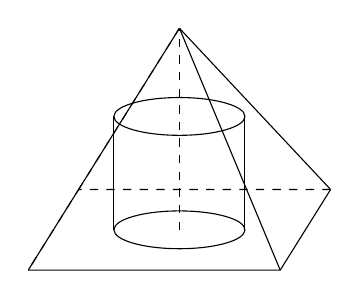
\begin{tikzpicture}[scale=0.32,font=\small]
\coordinate (A) at (-6,-1.6); \coordinate (B) at (4,-1.6); \coordinate (C) at (6,1.6); \coordinate (D) at (-4,1.6); \coordinate (S) at (0,8);
\draw (A)--(B)--(C); \draw[dashed] (C)--(D)--(A); \draw (S)--(A); \draw (S)--(B); \draw (S)--(C); \draw[dashed] (S)--(D);
\draw (0,0) ellipse (2.6 and 0.75); \draw (0,4.5) ellipse (2.6 and 0.75); \draw (-2.6,0)--(-2.6,4.5); \draw (2.6,0)--(2.6,4.5); \draw[dashed] (0,0)--(S);
\end{tikzpicture}}
\AB{Eng katta hajmli silindr hajmini toping.}{Silindr yon sirtining eng katta qiymatini toping.}}
\QQ{45}{Anvar bankdan yillik $20\%$ foiz stavkasi bilan $2$ yil muddatga $60$ mln söm miqdorida kredit oldi. Uning oylik tölovi quyidagi jadvalda körsatilgan.
\par\smallskip{\centering\renewcommand\arraystretch{1.25}\begin{tabular}{|c|c|c|c|c|}\hline
Oy & \shortstack{Qolgan asosiy\\summa} & \shortstack{Asosiy qarzdan\\tölov} & \shortstack{Foiz\\tölovi} & \shortstack{Jami oylik\\tölov}\\\hline
$1$ & $60\,000\,000$ & $2\,500\,000$ & $1\,000\,000$ & $3\,500\,000$\\\hline
$2$ & $57\,500\,000$ & $2\,500\,000$ & $958\,333{,}(3)$ & $3\,458\,333{,}(3)$\\\hline
$3$ & \ldots & \ldots & \ldots & \ldots\\\hline
$\vdots$ & $\vdots$ & $\vdots$ & $\vdots$ & $\vdots$\\\hline
$24$ & \ldots & \ldots & \ldots & \ldots\\\hline
\end{tabular}\par\smallskip}
\AB{Öninçi oyda tölanadigan oylik tölov (söm) qança böladi?}{Ikki yil mobaynidagi qöşilgan foiz tölovini (söm) toping.}}
\Javoblar{A B D A A B D C A B A A A D A C A C B B D D A A B C C C A A B D D A C}{\OK{36}{$4$}{$\dfrac47$}\OK{37}{$\dfrac\pi8$}{$0$}\OK{38}{$-1$}{$\dfrac{8\sqrt5}5$}\OK{39}{$2$}{$\dfrac{46}{15}$}\OK{40}{$\dfrac72$}{$9$}\OK{41}{$288$}{$96$}\OK{42}{$\sqrt2$}{$15^\circ$}\OK{43}{$1$}{$\sqrt{4+2\sqrt2}$}\OK{44}{$96$}{$54$}\OK{45}{$3\,125\,000$}{$12\,500\,000$}}
